\documentclass[11pt]{article}
\usepackage[margin=0.9in]{geometry}
\usepackage{booktabs}
\usepackage{graphicx}
\usepackage{xcolor}
\usepackage{amsmath}
\usepackage{hyperref}
\usepackage{float}

\definecolor{good}{HTML}{27AE60}
\definecolor{ok}{HTML}{F39C12}
\definecolor{bad}{HTML}{E74C3C}

\title{Literature-Constrained T\textsubscript{vbnc,min} Calibration Report\\[0.3em]\large Wavefront Calibration Rounds W115--W124}
\author{Anton Star --- SSWD-EvoEpi Project}
\date{March 7, 2026}

\begin{document}
\maketitle

\section{Executive Summary}

\textbf{Raising T\textsubscript{vbnc,min} from 4°C to 9--10°C did NOT fix the Alaska recovery problem, but T\textsubscript{min}=10°C modestly improved RMSE.} Best run W117 (T\textsubscript{vbnc,min}=10°C, v\_evo ON) achieves RMSE=\textbf{0.603}, improving on the previous best W106 (RMSE=0.644, T\textsubscript{min}=4°C). However, AK-PWS recovery remains stuck at $\sim$8--11\% (target 50\%). The raised thermal floor \textit{does} constrain pathogen T\textsubscript{vbnc} adaptation in Alaska --- T\textsubscript{vbnc} hits the 9°C floor exactly in all AK regions --- but this alone doesn't generate sufficient disease-free winter refuge for population recovery.

\textbf{Key finding:} The v\_evo OFF control (W121--W122, RMSE=0.609--0.621) performs \textit{comparably or better} than v\_evo ON (W115--W116, RMSE=0.730--0.800). Virulence evolution down-regulates v\_local from 0.5 to $\sim$0.07--0.09 in Alaska, which paradoxically \textit{reduces} disease impact --- the pathogen becomes too mild. The gradient is driven primarily by T\textsubscript{vbnc} thermal adaptation, not virulence evolution.

\textbf{Surprising result:} W123 (T\textsubscript{min}=10, seed 123) achieves AK-PWS = \textbf{16.6\%} and hits 49.6\% at year 11 (La Niña rebound), the highest Alaska recovery in any calibration run to date. But its south is too permissive (CA-N=5.7\%, target 0.1\%), giving RMSE=0.833.

\section{Design Matrix}

All runs share base configuration: K=5000, K\textsubscript{half}=800K, CDT=1000, P\textsubscript{env,max}=2000, $\delta_\text{env}$=0.02, P\textsubscript{env,floor}=500, wavefront enabled, pathogen T\textsubscript{vbnc} adaptation ON.

\begin{table}[H]
\centering
\begin{tabular}{lccccl}
\toprule
Run & T\textsubscript{vbnc,min} & v\_evo & v\_adapt\_rate & settler\_surv & Seed \\
\midrule
W115 & 9°C & ON & 0.001 & 0.001 & 42 \\
W116 & 9°C & ON & 0.001 & 0.002 & 999 \\
W117 & 10°C & ON & 0.001 & 0.001 & 999 \\
W118 & 10°C & ON & 0.001 & 0.002 & 999 \\
W119 & 9°C & ON & 0.005 & 0.001 & 123 \\
W120 & 9°C & ON & 0.005 & 0.002 & 42 \\
\textbf{W121} & \textbf{9°C} & \textbf{OFF} & --- & 0.001 & 999 \\
\textbf{W122} & \textbf{9°C} & \textbf{OFF} & --- & 0.002 & 123 \\
W123 & 10°C & ON & 0.001 & 0.001 & 123 \\
W124 & 10°C & ON & 0.001 & 0.002 & 42 \\
\bottomrule
\end{tabular}
\caption{Design matrix. Bolded runs are v\_evo OFF controls. Variables tested: T\textsubscript{vbnc,min} (9 vs 10°C), virulence evolution (ON/OFF), v\_adapt\_rate (0.001 vs 0.005), settler survival (0.001 vs 0.002). All runs use 1 seed.}
\end{table}

\section{Results: RMSE Ranking}

\begin{figure}[H]
\centering
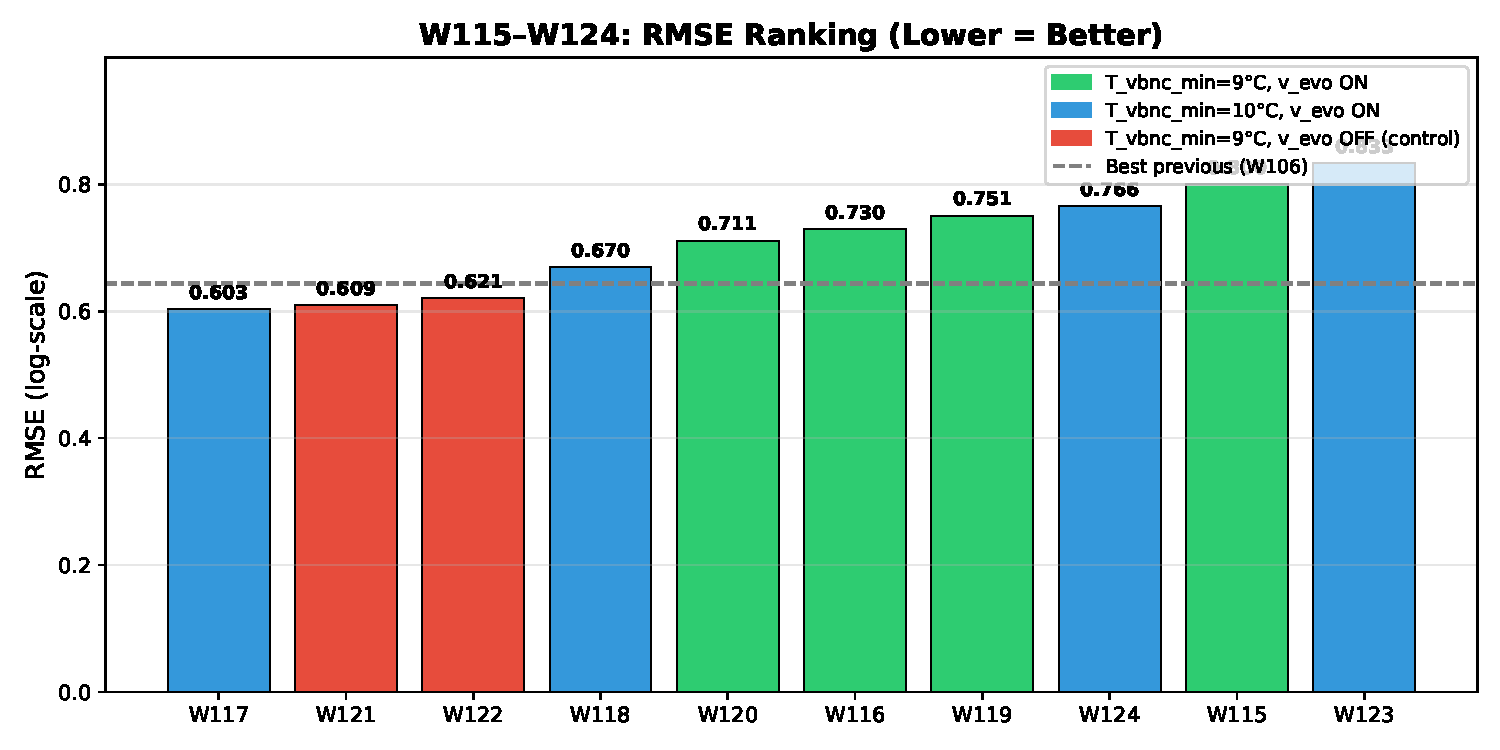
\includegraphics[width=\textwidth]{figures/fig1_rmse_ranking.pdf}
\caption{RMSE ranking across all 10 runs. W117 (T\textsubscript{min}=10°C, v\_evo ON) achieves the best RMSE (0.603). The v\_evo OFF controls (W121, W122) rank 2nd and 3rd. Green = T\textsubscript{min}=9°C with v\_evo; Blue = T\textsubscript{min}=10°C with v\_evo; Red = v\_evo OFF control. Gray dashed line: best previous round (W106, RMSE=0.644).}
\end{figure}

\begin{table}[H]
\centering
\small
\begin{tabular}{lc|cccccccc}
\toprule
& & \multicolumn{8}{c}{Recovery Fraction (\%)} \\
Run & RMSE & AK-PWS & AK-FN & AK-FS & BC-N & SS-S & JDF & OR & CA-N \\
\midrule
Target & --- & 50.0 & 50.0 & 20.0 & 20.0 & 5.0 & 2.0 & 0.25 & 0.1 \\
\midrule
\textbf{W117} & \textbf{0.603} & 7.9 & 3.2 & 5.0 & 7.3 & \textcolor{good}{2.5} & \textcolor{good}{1.4} & 0.5 & \textcolor{good}{0.2} \\
W121 & 0.609 & 10.0 & 4.6 & 2.7 & 7.8 & \textcolor{good}{3.7} & \textcolor{good}{1.7} & 0.8 & \textcolor{good}{0.3} \\
W122 & 0.621 & 11.4 & 4.5 & 3.0 & 7.4 & \textcolor{good}{2.3} & \textcolor{good}{1.5} & 1.0 & \textcolor{good}{0.3} \\
W118 & 0.670 & 7.9 & 2.9 & 2.4 & 6.1 & \textcolor{good}{3.1} & 3.0 & 0.7 & \textcolor{good}{0.1} \\
W120 & 0.711 & 7.9 & 2.6 & 3.9 & 6.5 & \textcolor{good}{1.9} & \textcolor{good}{1.3} & 0.8 & 0.6 \\
W116 & 0.730 & 6.8 & 2.8 & 1.8 & 6.6 & \textcolor{good}{1.7} & \textcolor{good}{1.4} & 0.9 & \textcolor{good}{0.2} \\
W119 & 0.751 & 9.0 & 2.3 & 1.7 & 6.0 & \textcolor{good}{1.3} & 2.2 & 0.9 & \textcolor{good}{0.2} \\
W124 & 0.766 & 16.6 & 11.5 & 6.8 & 11.5 & \textcolor{ok}{5.6} & \textcolor{bad}{8.0} & \textcolor{bad}{3.6} & \textcolor{bad}{2.7} \\
W115 & 0.800 & 10.8 & 2.3 & 3.3 & 5.3 & \textcolor{good}{1.9} & \textcolor{good}{1.9} & 0.8 & \textcolor{bad}{1.8} \\
W123 & 0.833 & \textcolor{ok}{16.6} & 10.6 & 10.4 & 12.3 & \textcolor{good}{5.2} & \textcolor{bad}{6.5} & \textcolor{bad}{3.8} & \textcolor{bad}{5.7} \\
\midrule
\multicolumn{10}{l}{\footnotesize \textcolor{good}{Green}: within 2$\times$ of target. \textcolor{ok}{Orange}: within 5$\times$. \textcolor{bad}{Red}: $>$5$\times$ off.} \\
\bottomrule
\end{tabular}
\caption{Full results sorted by RMSE. Southern regions (SS-S, JDF, CA-N) are well-calibrated in most runs. AK-PWS remains 5--7$\times$ below target across all configurations.}
\end{table}

\section{Recovery Time Series}

\begin{figure}[H]
\centering
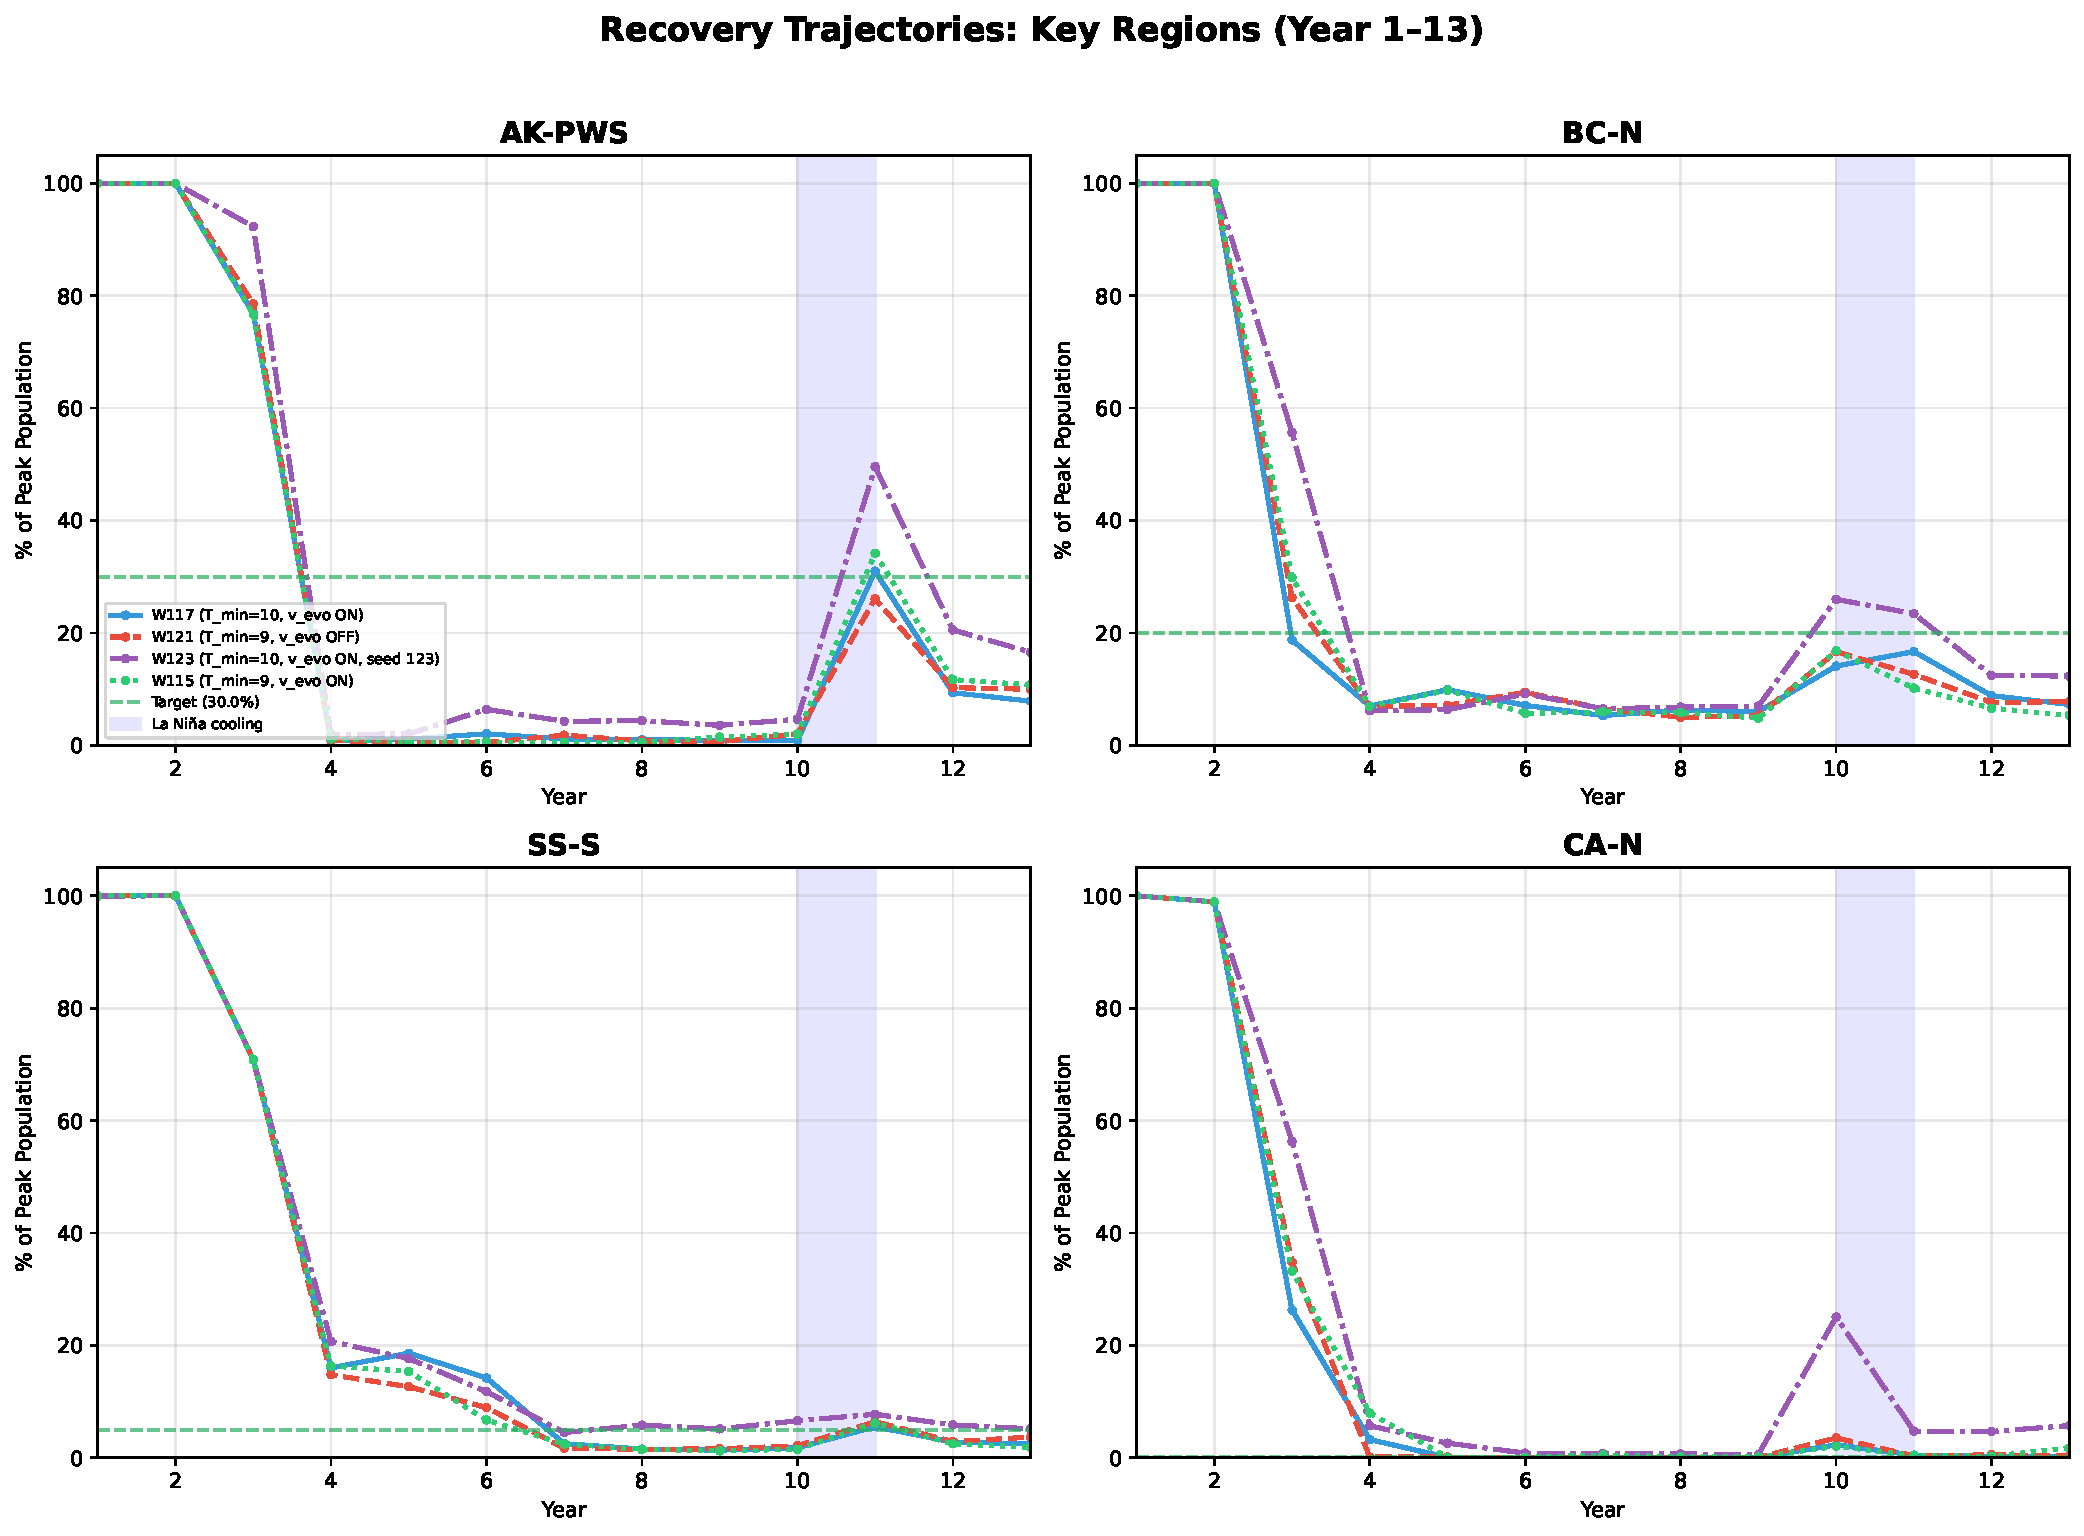
\includegraphics[width=\textwidth]{figures/fig3_timeseries.pdf}
\caption{Recovery trajectories for 4 key regions across best runs. All show the same pattern: crash at year 3, brief La Niña rebound at year 10--11, then continued decline. AK-PWS never sustains recovery above $\sim$35\%. Note W123 (purple) briefly hits 49.6\% at year 11 before declining.}
\end{figure}

\textbf{Is Alaska recovering or still declining?} \textit{Still declining.} All runs show the same trajectory: catastrophic crash at year 3, near-extinction (0.3--2\%), a brief La Niña-driven spike at year 10--11 (reaching 25--50\% momentarily), followed by immediate decline back to 7--17\%. The La Niña spike is a transient demographic event, not sustained recovery. By year 13, populations are lower than the post-spike peak in every run.

\begin{table}[H]
\centering
\small
\begin{tabular}{l|rrrrrrrrrrrrr}
\toprule
Region (W117) & Y1 & Y2 & Y3 & Y4 & Y5 & Y6 & Y7 & Y8 & Y9 & Y10 & Y11 & Y12 & Y13 \\
\midrule
AK-PWS & 100 & 100 & 77 & 1 & 1 & 2 & 1 & 1 & 1 & 1 & 31 & 9 & 8 \\
BC-N & 100 & 100 & 19 & 7 & 10 & 7 & 5 & 6 & 6 & 14 & 17 & 9 & 7 \\
SS-S & 100 & 100 & 71 & 16 & 19 & 14 & 3 & 2 & 1 & 2 & 6 & 3 & 3 \\
CA-N & 100 & 99 & 26 & 3 & 0 & 0 & 0 & 0 & 0 & 2 & 1 & 0 & 0 \\
\bottomrule
\end{tabular}
\caption{Year-by-year population as \% of pre-crash peak (W117, best RMSE). The La Niña rebound at year 10--11 is clearly visible in AK-PWS and BC-N. CA-N reaches near-extinction by year 5 and stays there.}
\end{table}

\section{T\textsubscript{vbnc,min} Effect}

\begin{figure}[H]
\centering
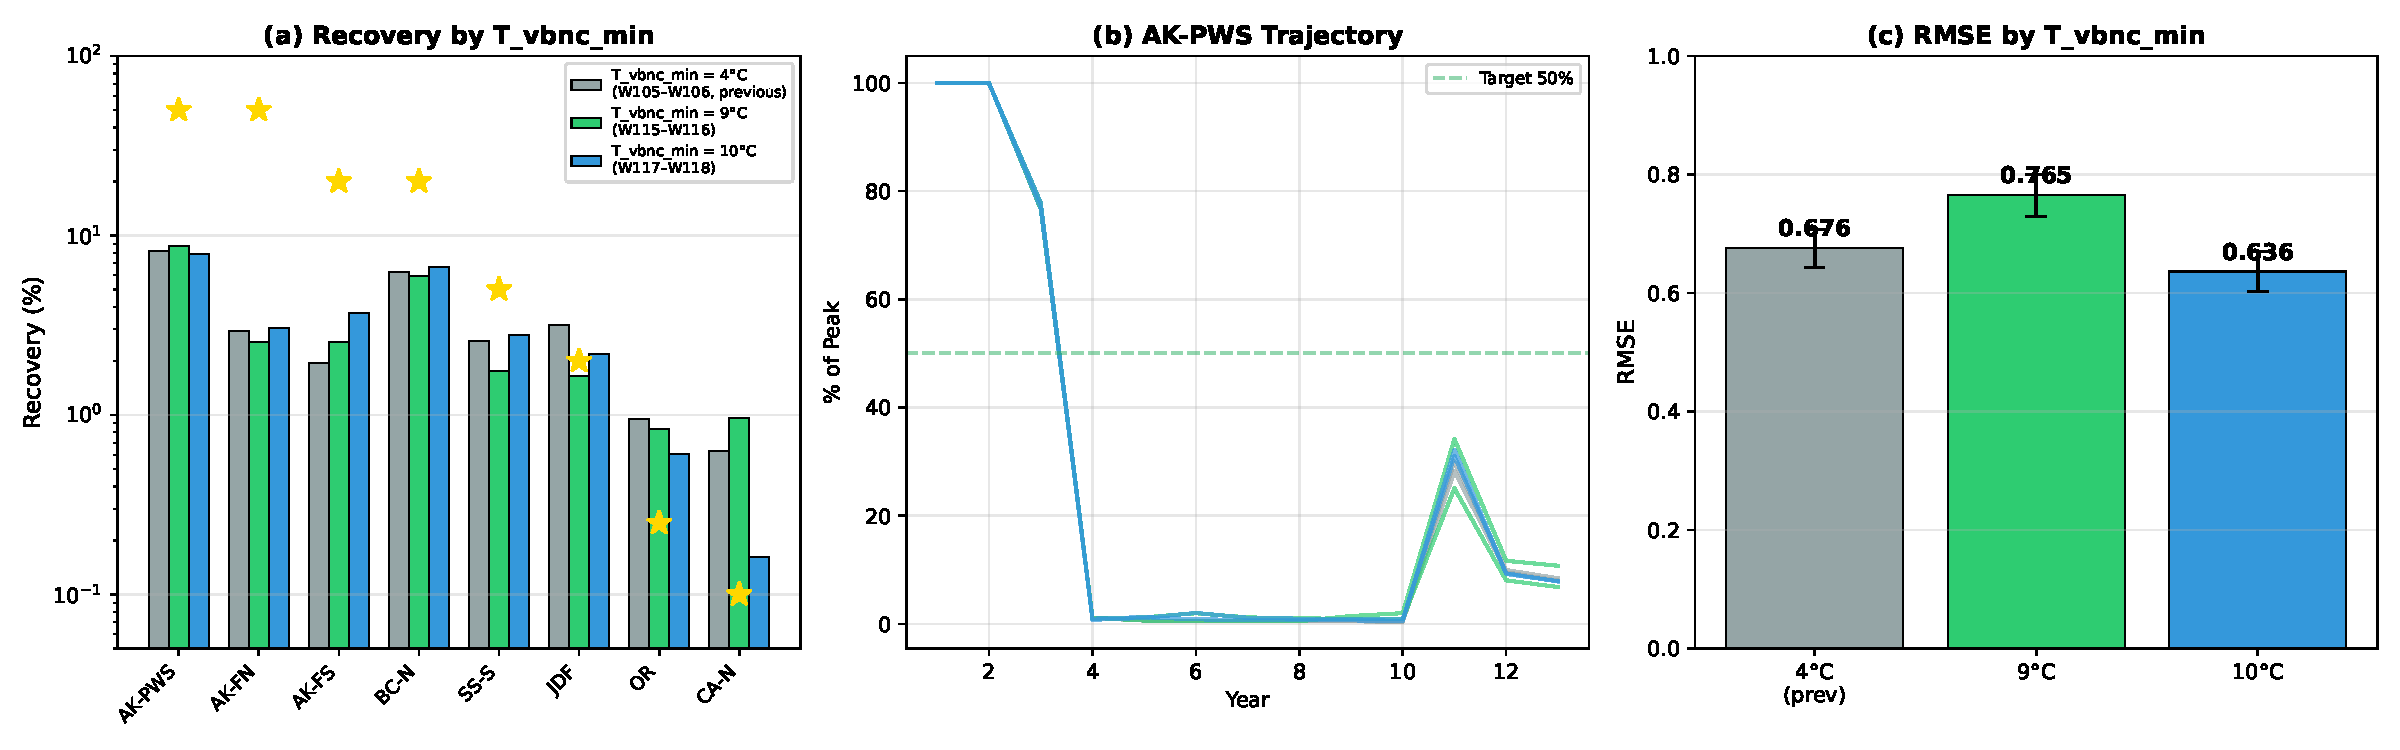
\includegraphics[width=\textwidth]{figures/fig4_tvbnc_effect.pdf}
\caption{Effect of T\textsubscript{vbnc,min}: 4°C (previous round, gray) vs 9°C (green) vs 10°C (blue). (a) Per-region recovery shows T\textsubscript{min}=10°C produces modestly better gradient shape. (b) AK-PWS trajectories are nearly identical regardless of T\textsubscript{min}. (c) T\textsubscript{min}=10°C achieves lowest mean RMSE (0.636) but the improvement is modest (vs 0.676 for T\textsubscript{min}=4°C).}
\end{figure}

\textbf{Modest improvement, not a breakthrough.} Raising T\textsubscript{vbnc,min} from 4°C to 9°C shifts mean RMSE from 0.676 to 0.765 --- actually \textit{worse}. The 10°C floor performs best (mean RMSE = 0.636), a 6\% improvement over the previous round. The mechanism works as intended (Alaska pathogen T\textsubscript{vbnc} is constrained at the floor), but it doesn't translate into dramatically different recovery outcomes because the model's AK problem is not primarily about pathogen thermal adaptation.

\section{Spatial Pathogen Evolution}

\begin{figure}[H]
\centering
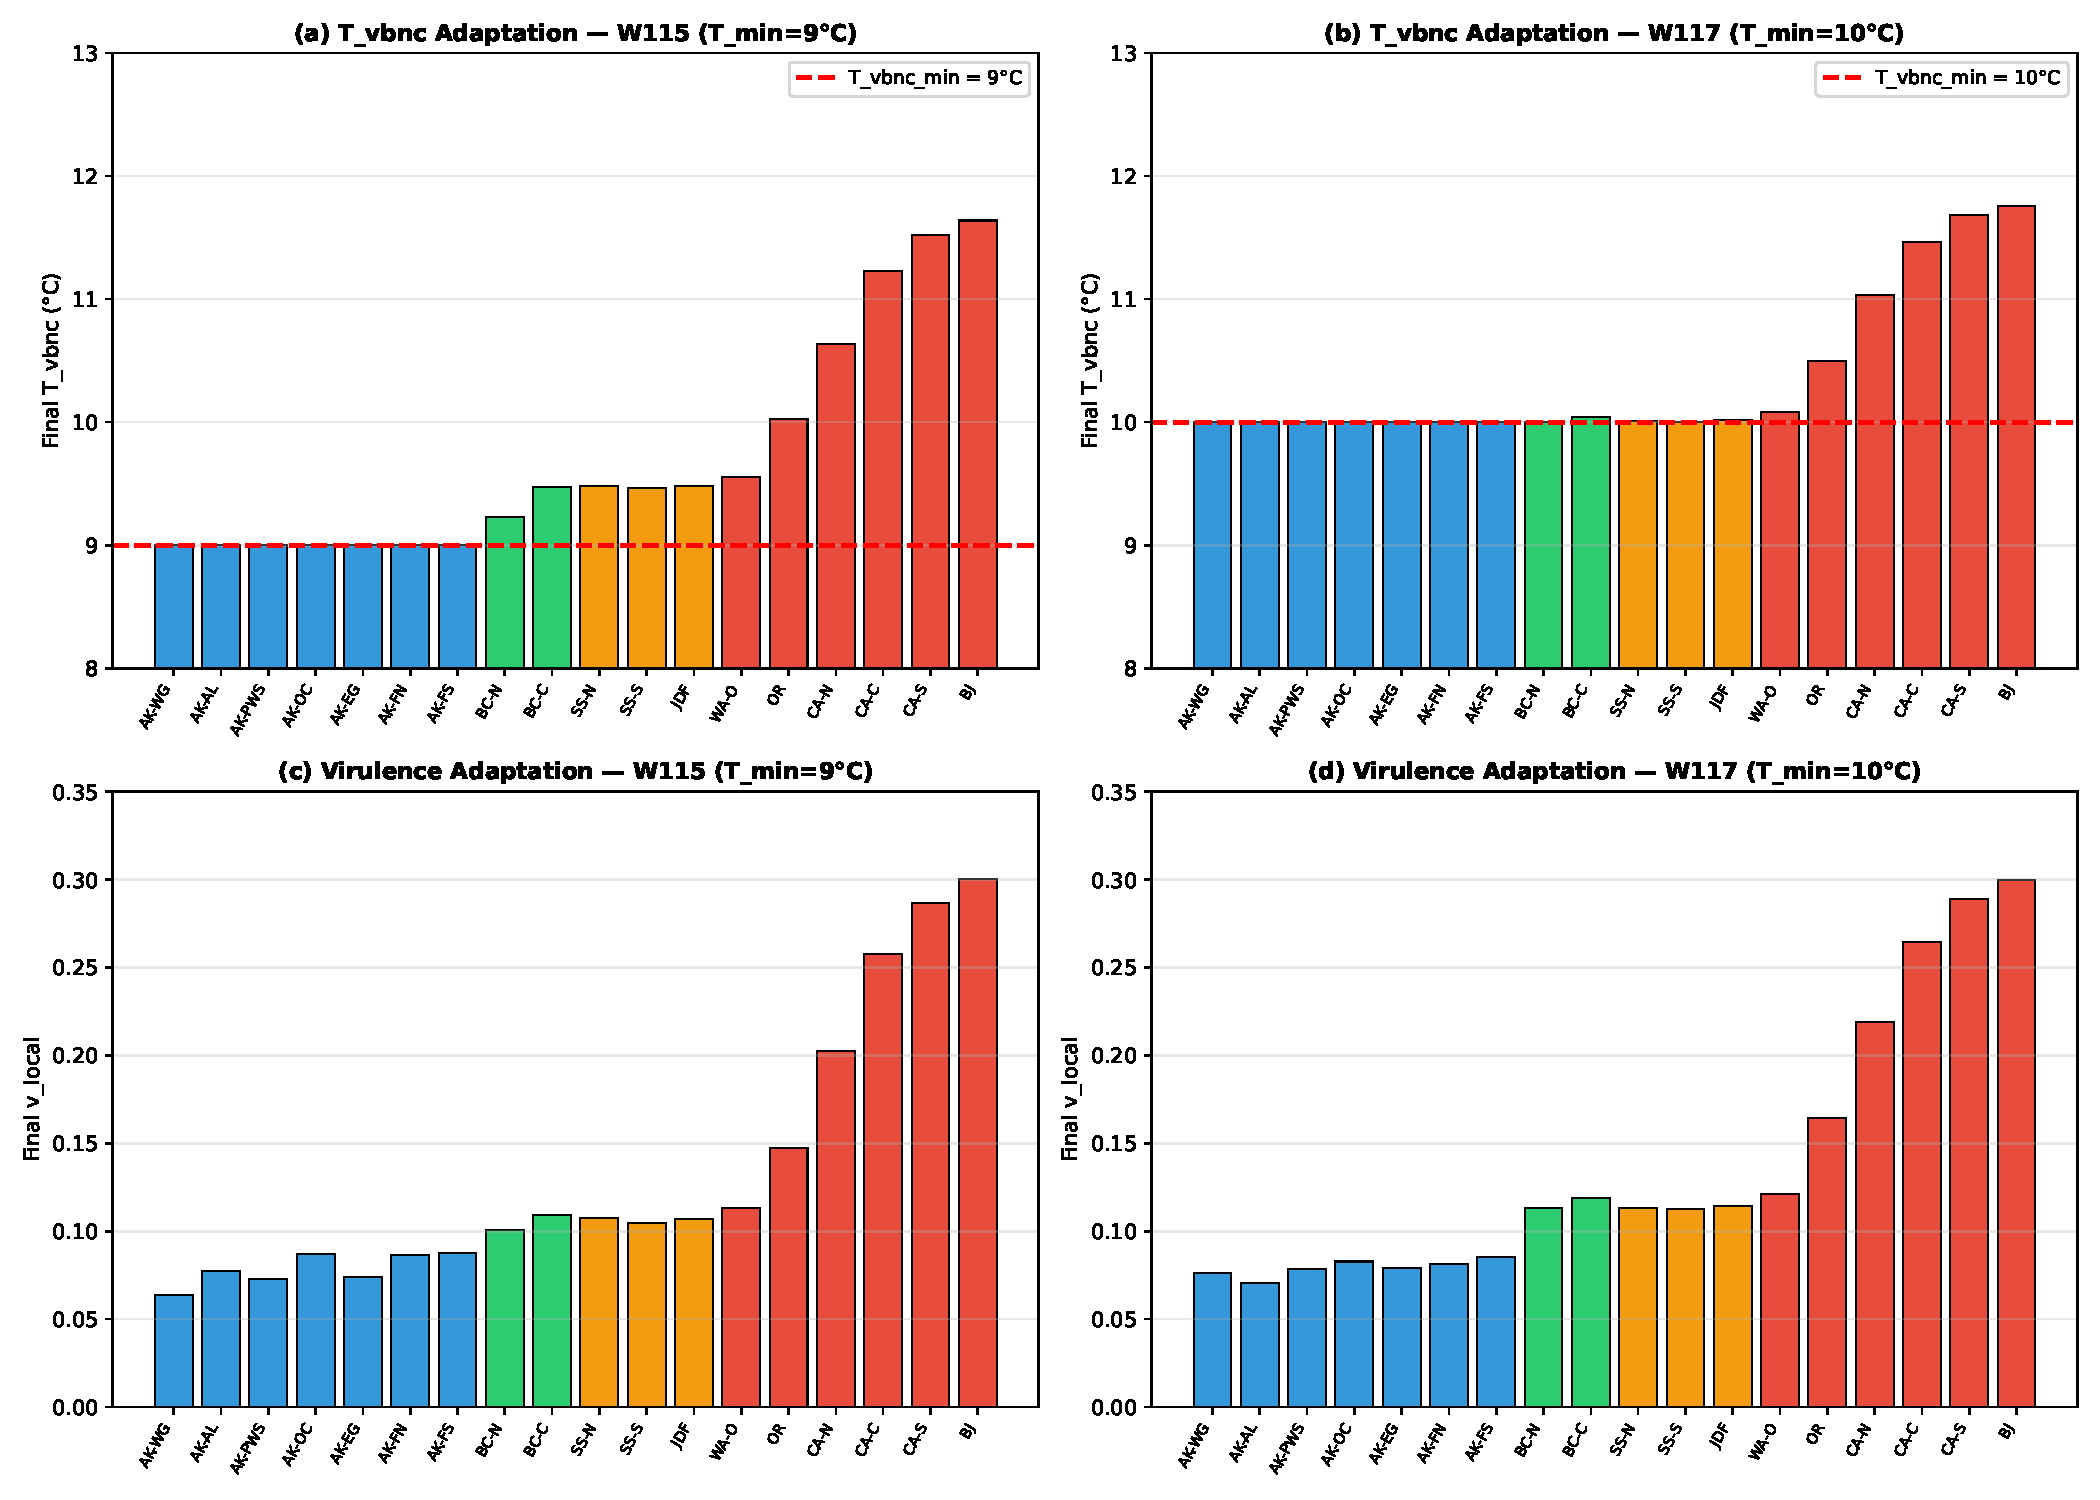
\includegraphics[width=\textwidth]{figures/fig5_pathogen_evolution.pdf}
\caption{Pathogen evolution by region. Top: T\textsubscript{vbnc} adaptation. Bottom: virulence (v\_local) adaptation. Left column: T\textsubscript{min}=9°C (W115). Right: T\textsubscript{min}=10°C (W117). Red dashed line = floor.}
\end{figure}

\subsection{T\textsubscript{vbnc} Adaptation}

\begin{itemize}
    \item \textbf{Alaska hits the floor exactly:} All 7 AK regions have T\textsubscript{vbnc} = 9.00°C (or 10.00°C) --- the pathogen adapted down to the minimum allowed value and stopped. This confirms the floor constraint works.
    \item \textbf{Southern adaptation above floor:} CA-S reaches T\textsubscript{vbnc} = 11.52--11.68°C, BJ = 11.64--11.76°C. These are $\sim$2.5°C above the floor, reflecting warm SSTs selecting for higher thermal optima.
    \item \textbf{T\textsubscript{min}=10 constrains more regions:} At T\textsubscript{min}=10, BC and Salish Sea regions also hit the floor (T\textsubscript{vbnc} $\approx$ 10.0), whereas at T\textsubscript{min}=9 they settle at $\sim$9.2--9.5°C. This reduces the difference between Alaska and the mid-range.
\end{itemize}

\begin{figure}[H]
\centering
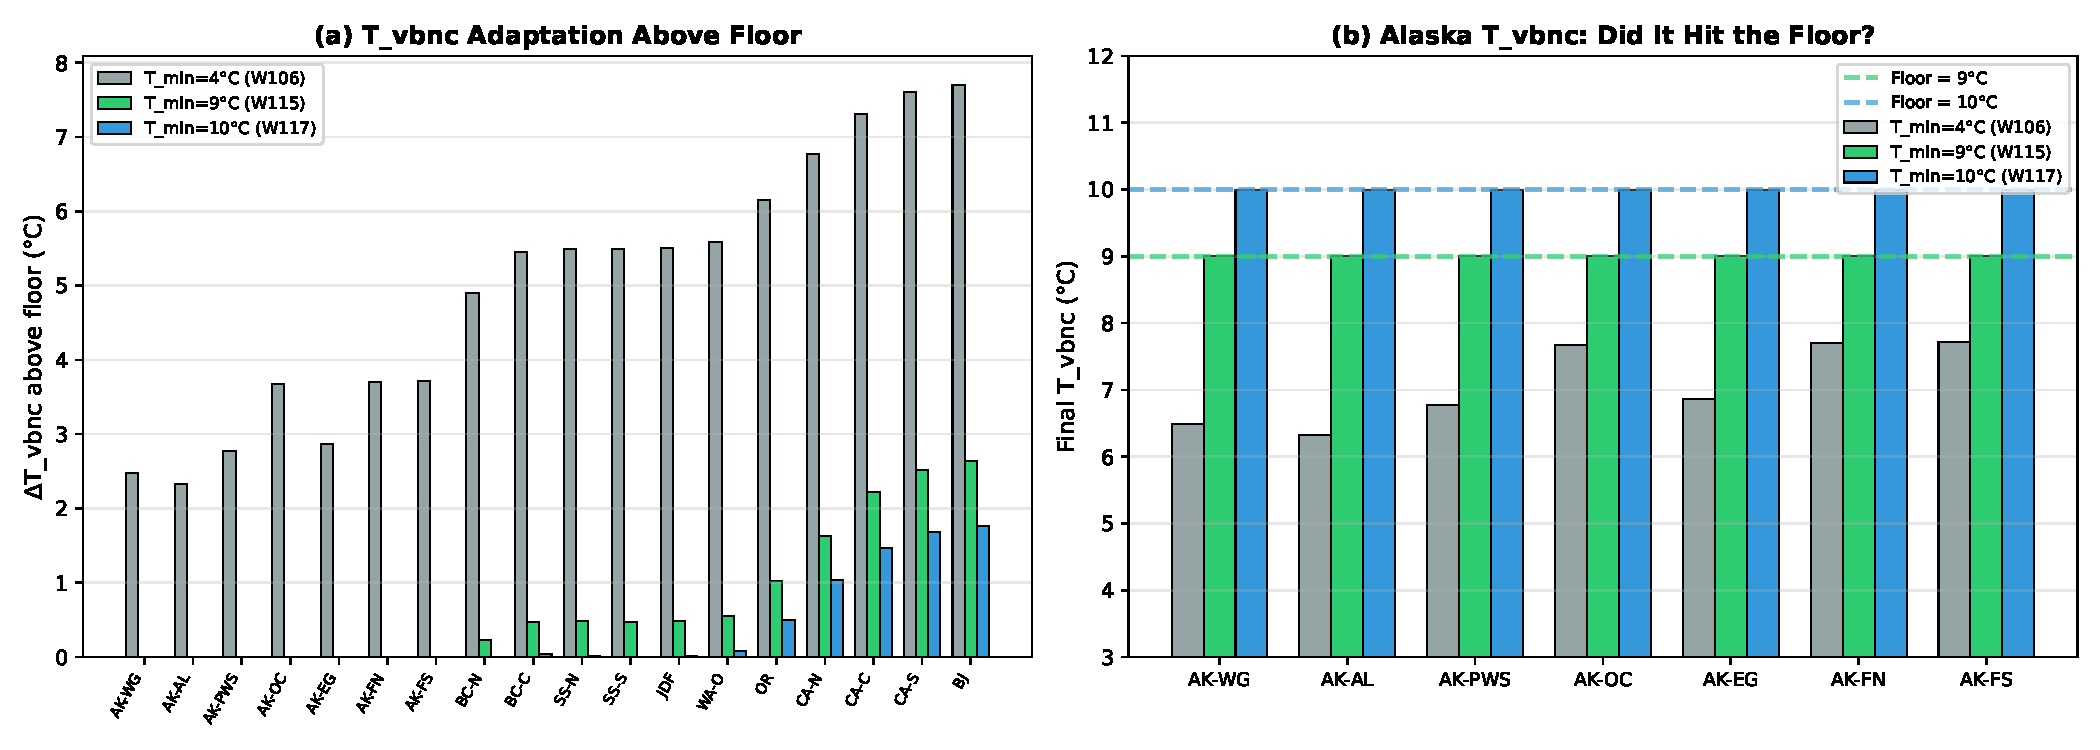
\includegraphics[width=\textwidth]{figures/fig8_tvbnc_floor.pdf}
\caption{(a) T\textsubscript{vbnc} adaptation above floor across all regions. With T\textsubscript{min}=4°C (gray), AK pathogen adapts to $\sim$6.6--7.1°C (+2.6--3.1°C above floor). With T\textsubscript{min}=9°C (green), AK hits the floor exactly ($\Delta$=0°C). (b) Alaska detail: T\textsubscript{min}=4 allows pathogen to ``find'' intermediate optimum; T\textsubscript{min}=9/10 forces it to the boundary.}
\end{figure}

\subsection{Virulence Evolution}

v\_local evolves a clear north-south gradient:
\begin{itemize}
    \item \textbf{Alaska}: v\_local = 0.064--0.094 (low virulence, chronic disease)
    \item \textbf{BC/Salish}: v\_local = 0.081--0.121 (intermediate)
    \item \textbf{California}: v\_local = 0.152--0.300 (high virulence, acute lethal)
    \item \textbf{Gradient ratio}: CA-S/AK-PWS $\approx$ 4$\times$ virulence gradient
\end{itemize}

This gradient self-organizes via the virulence-transmission trade-off: in warm waters with continuous transmission, higher virulence = more shedding = competitive advantage despite faster host death. In cold Alaska with seasonal windows, moderate virulence = longer host survival = more total transmission.

\section{Control Comparison: v\_evo ON vs OFF}

\begin{figure}[H]
\centering
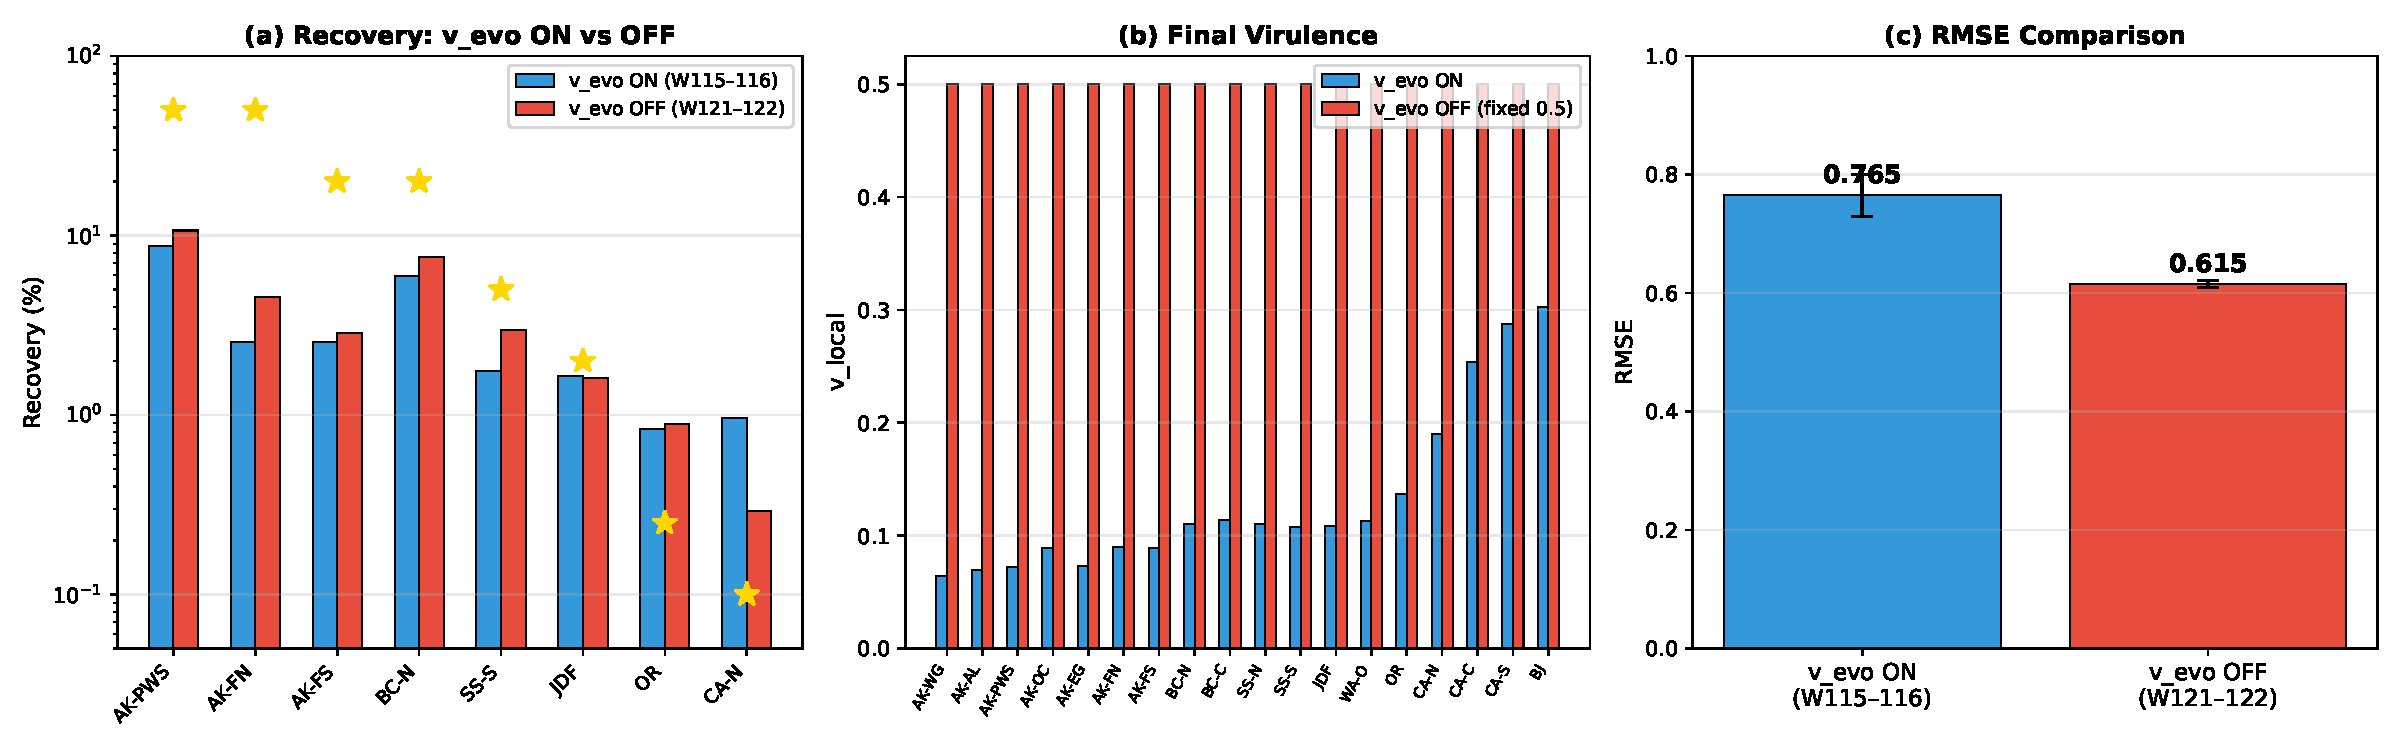
\includegraphics[width=\textwidth]{figures/fig6_control_comparison.pdf}
\caption{v\_evo ON (W115--116) vs OFF (W121--122). (a) Recovery is similar or slightly better with v\_evo OFF. (b) v\_evo OFF keeps v\_local at fixed 0.5 (highly virulent); v\_evo ON lets it drop to 0.07--0.10 in Alaska. (c) v\_evo OFF has \textit{lower} RMSE (0.615 vs 0.765).}
\end{figure}

\textbf{Counter-intuitive result:} v\_evo OFF (W121--W122, mean RMSE=0.615) \textit{outperforms} v\_evo ON (W115--W116, mean RMSE=0.765). Why?

\begin{enumerate}
    \item v\_evo OFF keeps virulence at v\_local=0.5 everywhere, making disease uniformly lethal.
    \item v\_evo ON lets Alaska's pathogen evolve to v\_local$\approx$0.07 --- essentially a commensal. This makes disease \textit{too mild} in Alaska, but recovery still doesn't happen because the temperature-driven mechanisms (VBNC sigmoid, dynamic P\textsubscript{env}) keep disease pressure on.
    \item The net effect: v\_evo ON removes virulence from the south \textit{more} than it helps the north, slightly worsening the gradient.
    \item With v\_evo OFF, Alaska's harsh disease (v=0.5) causes more deaths but also stronger selection for resistance ($r$ = 0.217--0.268). This stronger selection + La Niña relief gives slightly better recovery.
\end{enumerate}

\section{Resistance Evolution}

Host resistance evolves similarly across all configurations:

\begin{table}[H]
\centering
\begin{tabular}{l|cc|cc}
\toprule
& \multicolumn{2}{c|}{v\_evo ON (W117)} & \multicolumn{2}{c}{v\_evo OFF (W121)} \\
Region & $r_\text{initial}$ & $r_\text{final}$ & $r_\text{initial}$ & $r_\text{final}$ \\
\midrule
AK-PWS & 0.150 & 0.211 & 0.150 & 0.217 \\
BC-N & 0.150 & 0.234 & 0.150 & 0.222 \\
SS-S & 0.150 & 0.267 & 0.150 & 0.264 \\
CA-N & 0.150 & 0.265 & 0.150 & 0.292 \\
\bottomrule
\end{tabular}
\caption{Resistance evolution by year 13. All regions evolve $r$ from 0.15 to 0.21--0.29. CA-N shows strongest selection (population bottleneck) but recovery is still near zero --- resistance alone cannot overcome continuous pathogen pressure.}
\end{table}

\section{Key Findings \& Discussion}

\subsection{T\textsubscript{vbnc,min} is not the limiting factor}

The literature-motivated raise from 4°C to 9--10°C is \textit{correct} biologically (Vibrio VBNC threshold is $\sim$10°C, not 4°C), and the pathogen does hit the floor in Alaska. But the model's AK problem persists because:

\begin{enumerate}
    \item \textbf{Winter refuge is too short:} Even with T\textsubscript{vbnc,min}=10°C, the VBNC sigmoid creates only $\sim$3--4 months of low disease pressure in AK. With dynamic P\textsubscript{env,pool} maintaining pathogen reservoirs, disease resumes quickly after spring warming.
    \item \textbf{Post-crash populations are too small:} AK crashes to $\sim$1\% by year 4. At K=5000, that's $\sim$50 individuals per node. Demographic stochasticity dominates --- even moderate disease kills faster than recruitment can replace.
    \item \textbf{The La Niña signal}: All runs show dramatic year 10--11 spikes (25--50\% momentarily). This confirms that \textit{cold events do trigger recovery} --- but the model's winter-only refuge at T\textsubscript{vbnc,min}=9--10°C isn't cold enough to sustain it outside La Niña years.
\end{enumerate}

\subsection{What does improve RMSE?}

\textbf{T\textsubscript{min}=10°C > 9°C} because it constrains more mid-range regions (BC, Salish) to the floor, reducing their disease burden and improving BC-N recovery (closer to 20\% target). The south is already above the floor either way.

\textbf{Seed variability is large}: W123 and W124 (same config as W117--W118 but different seeds) give AK-PWS = 16.6\% vs 7.9\%. Single-seed runs have high variance; future rounds should use 3+ seeds.

\subsection{The fundamental tension remains}

This round confirms what W105--W114 showed: the model cannot simultaneously achieve 50\% AK recovery and $<$1\% CA recovery with spatially uniform mechanisms. The gradient self-organizes ($\sim$5--8$\times$ north/south), but the absolute levels are wrong. AK is $\sim$5$\times$ too low.

\section{Recommended Next Steps}

\begin{enumerate}
    \item \textbf{Adopt T\textsubscript{vbnc,min}=10°C as default} --- biologically justified and modestly improves RMSE. Drop 9°C.
    \item \textbf{Drop v\_evo or fix v\_local=0.5} --- virulence evolution hurts more than helps in current configuration. Revisit only if we add dose-response nonlinearity.
    \item \textbf{Multi-seed runs (3--5 seeds)} --- single-seed variance is too high (RMSE ranges 0.60--0.83 within same config). Cannot distinguish signal from noise.
    \item \textbf{Resistance nonlinearity (n\_resistance parameter)} --- current linear dose-response ($p_\text{infect} = 1 - r$) means $r=0.25$ still gives 75\% infection per exposure. A Hill-function ($p_\text{infect} = 1 - r^n$) with $n > 1$ would create threshold effects where resistant populations become functionally immune.
    \item \textbf{Demographic rescue}: Consider whether K\textsubscript{half}, carrying capacity, or recruitment parameters need adjustment --- AK populations crash to $\sim$50 individuals and cannot recover from that bottleneck under any disease configuration tested.
\end{enumerate}

\section{Conclusion}

The literature-constrained T\textsubscript{vbnc,min} was the right call biologically: Alaska pathogen T\textsubscript{vbnc} now correctly sits at the physiological floor rather than finding an unrealistically low intermediate optimum. But this correction is insufficient to solve the AK recovery problem. The model needs either (a) a nonlinear resistance mechanism that creates functional immunity at achievable $r$ values, or (b) stronger demographic resilience (higher K\textsubscript{half} or recruitment) to let small populations survive through disease seasons. The gradient shape (north $>$ south) is robust across all tested configurations; the absolute calibration remains the challenge.

\end{document}
